\documentclass[a4paper,10 pt]{article}

%% Language and font encodings
\usepackage[spanish,es-tabla]{babel}
\usepackage[utf8]{inputenc}
\usepackage[T1]{fontenc}
\usepackage{cite}
\usepackage{amsmath, amsthm, amssymb, amsfonts} 
\usepackage[mathscr]{eucal}
\usepackage{ulem} % subrayar, tachar
\usepackage{hyperref} % para el url
\usepackage{multirow, array} % para las tablas
\usepackage{float} % para tablas [H]
\usepackage{graphicx} % graficos
\usepackage{titlesec} %subsubsubsection
\usepackage[usenames]{color} %palabras con color
\usepackage{lscape} % texto horizontal
\usepackage{pdflscape} % hoja horizontal
\usepackage{booktabs} %tabla con puntos
\usepackage{longtable}
\usepackage{url}

% Break long url
\makeatletter
\g@addto@macro{\UrlBreaks}{\UrlOrds}
\makeatother

\newcolumntype{P}[1]{>{\centering\arraybackslash}p{#1}}
\newcolumntype{M}[1]{>{\centering\arraybackslash}m{#1}}
\newcolumntype{L}[1]{>{\raggedleft\arraybackslash}p{#1}}
\newcolumntype{R}[1]{>{\raggedright\arraybackslash}p{#1}}

%ppppppppppppppppppppppppppppppppppppppppppppppppppppppppppppppppppppppppppppppp

%% Sets page size and margins
\usepackage[a4paper,top=2cm,bottom=2cm,left=2cm,right=2cm,marginparwidth= 1.5cm]{geometry}
  
\title{\textbf{Retrospectiva - Sprint 1}}

% Chicos, porfavor incluyan sus nombres en orden alfabetico
\author{\textbf{Grupo 7}\\
        \normalsize Valeria Huepa Ducuara\\
        \normalsize Juan José Peña Becerra\\
        \normalsize Carlos Daniel Rincón Mora\\
        \normalsize Guiselle Tatiana Zambrano Penagos}
\date{\today}

\begin{document}

\maketitle

Para el desarrollo de la retrospectiva nos reunimos a través de la herramienta
Meet y elaboramos una tablero en Trello, donde agregamos 3 listas (Went Well,
Needs To Change and Action Items) y en ellas agregamos tarjetas
mientras discutíamos sobre nuestro desempeño en el sprint. \\

\textbf{Link del tablero:} \url{https://trello.com/invite/b/uwbIx1JY/b014c88adcf4b35e23fef7e0ca041235/sprint-retrospective-1}\\

El resumen de los puntos discutidos en dicha reunión será mostrados a
continuación.

\section{¿Qué salió bien en el Sprint?}

\begin{itemize}
    \item Nos organizarnos y definimos las tareas a realizar durante el sprint.
    \item Las plantillas creadas en el front\_end se adaptan bien a los mockups
    elaborados en el sprint 0.
    \item Aprendimos a utilizar Kanban para seguir el desarrollo de los
    repositorios en la organización.
    \item Aprendimos a utilizar Slack e integrarlo con Github para poder seguir
    los cambios realizados sobre los repositorio y crear un ambiente de
    discusión más cómodo.
    \item Entendemos la funcionalidad de las ramas utilizadas en el
    repositorio.
    \item Consideramos que elegimos bien los Frameworks.
    \item Logramos suplir las deudas técnicas del sprint 0.
\end{itemize}{}

\section{¿Qué podría mejorarse?}

\begin{itemize}
    \item Aprender con más profundidad los lenguajes y los frameworks
    seleccionados.
    \item Mejorar la división de tareas.
    \item Utilizar mejor las herramientas git y github.
    \item Evaluar de una mejor forma el esfuerzo requerido para cada tarea
    definida.
    \item La constancia en el desarrollo de las tareas en todo el equipo.
    \item Mejorar el diálogo entre los integrantes para que las tareas creadas
    por cada miembro sean compatibles entre ellas.
\end{itemize}{}

\section{¿Qué nos comprometeremos a mejorar en el próximo Sprint?}

\begin{itemize} 
    \item Definiremos las tareas y la asignación de estas a los miembros
    del equipo al inicio del sprint.
    \item Organizaremos las reuniones al inicio del sprint.
    \item Vamos a reunirnos con más frecuencia para discutir nuestros avances,
    propuestas o inconvenientes con el desarrollo de las tareas asignadas.
    \item Integrar a Slack otras herramientas que faciliten el trabajo del
    equipo, como por ejemplo Google Drive, Google Calendar y Trello.
    \item Mejorar el Kanban utilizado en el sprint y establecer un esquema para
    definir las tareas.
    \item Realizar las tareas asignadas de manera constante.
    \item Familiarizarnos más con el editor de código y encontrar complementos
    que faciliten el proceso de desarrollo dentro de este.
    \item Definir un espacio en donde podamos adjuntar recursos de aprendizaje
    relacionados con los lenguajes y framewors a utilizar.
    \item Evaluar el desempeño grupal cada semana y crear estrategias de
    mejora.
    \item Cada miembro del equipo trabajará en el front-end y back-end.
\end{itemize}{}

\section{Capturas de pantalla}

\begin{figure}[H]
    \centering
    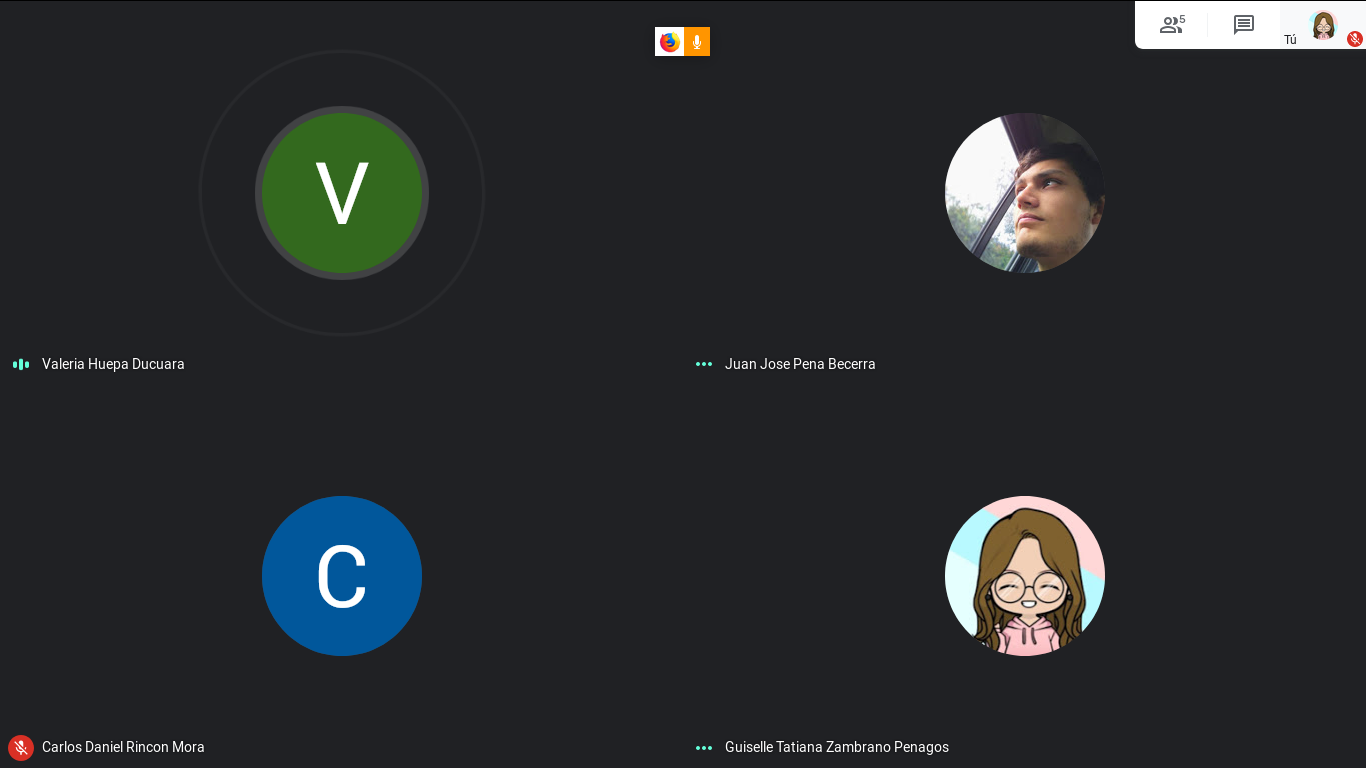
\includegraphics[scale = 0.25]{images/equipo.png}
    \caption{Captura de la videollamada}
    \label{f00}
\end{figure}{}

\begin{figure}[H]
    \centering
    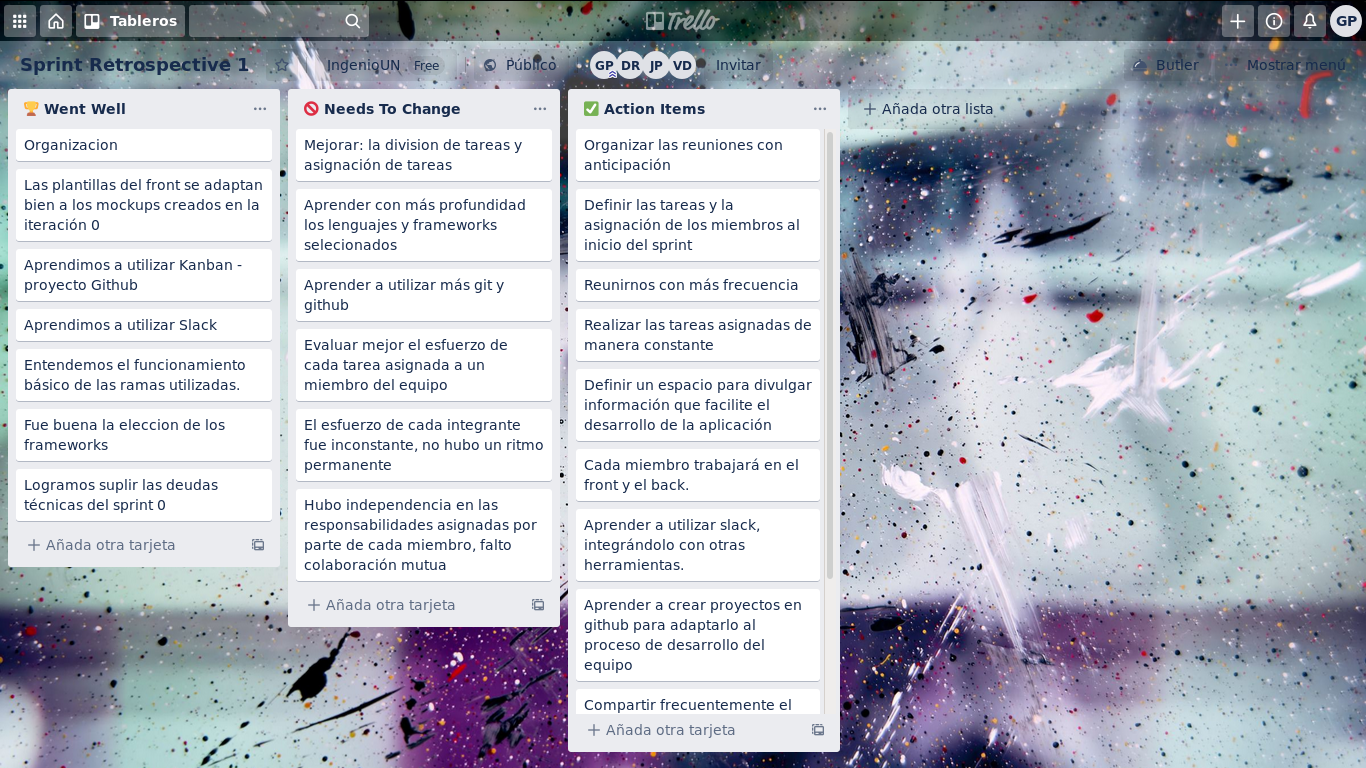
\includegraphics[scale = 0.25]{images/tablero.png}
    \caption{Tablero de trello}
    \label{f01}
\end{figure}{}

\end{document}
